\section[Beam Position Monitors]{Beam Position Monitors}

To determine the position and the direction of the beam on the experimental 
target point, two Beam Position Monitors (BPMs) are located at distances 7.524 m 
(IPM1H03A) and 1.286 m (IPM1H03B) upstream of the target position. 
The BPMs consist of a 4-wire antenna array of open ended thin wire striplines 
tuned to the fundamental RF frequency of 1.497 GHz of the beam ~\cite{bi:bar90}. The 
standard difference-over-sum technique is then used ~\cite{bi:HW} to determine the 
relative position of the beam to within 100 microns for currents
above 1 $\mu $A. The absolute  position of the BPMs can be calibrated with respect to the 
scanners (superharps) which are located adjacent to each of the BPMs (IHA1H03A 
at 7.353 m and IHA1H03B at 1.122 m upstream of the target). 
\infolevone{The schematic of the  readout electronics is shown in Figure ~\ref{fig:bpmel}.}
The position information from the 
BPMs can be recorded in three different ways:

\infolevone{
\begin{figure}[hp]
\begin{center}
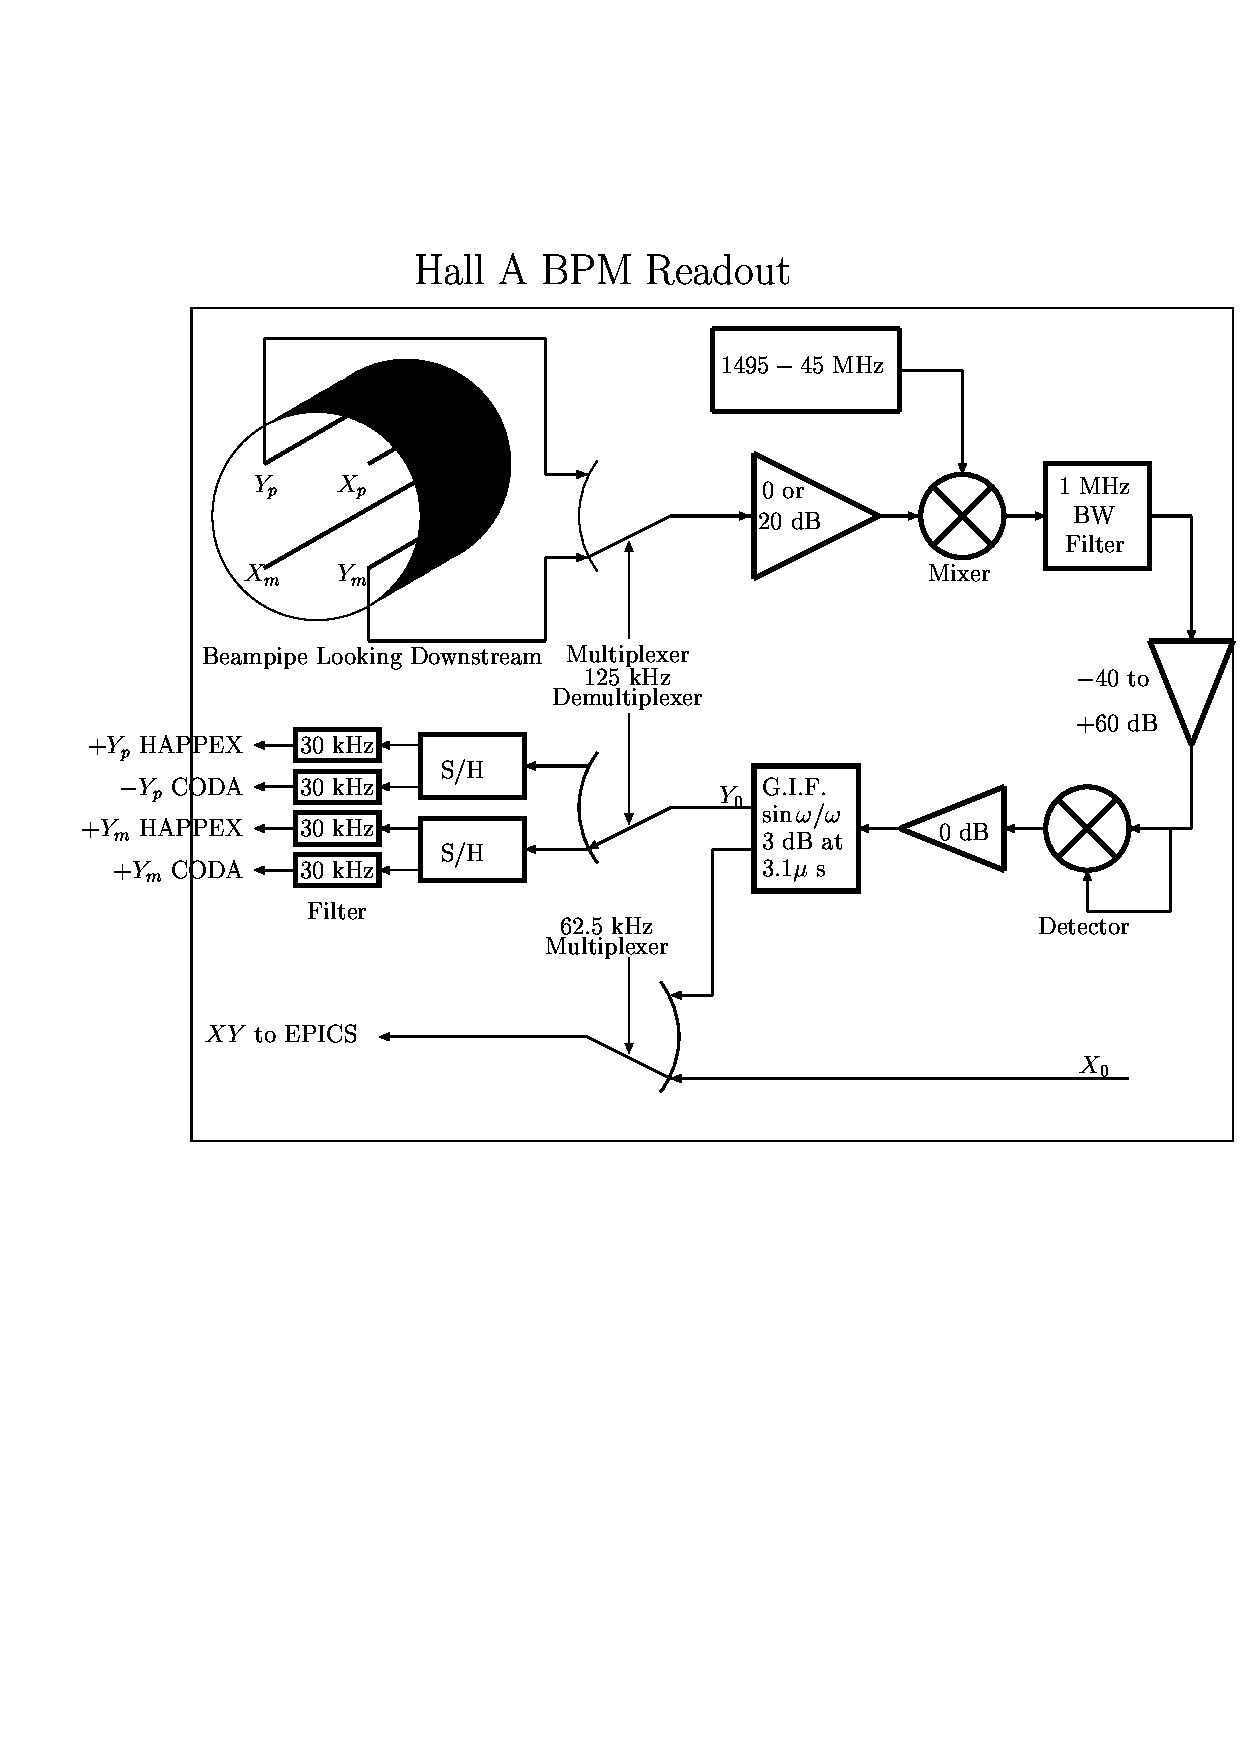
\includegraphics[angle=0,width=15cm]{BPM_fig}
{\linespread{1.}
\caption[Beamline: BPM Readout Electronics]{Schematic of the BPM readout
electronics}
\label{fig:bpmel}}
\end{center}
\end{figure}
}

1. The averaged position over 0.3 seconds is logged into the EPICS~\cite{EPICSwww} database (1 
Hz updating frequency) and injected into the datastream every 3-4 seconds, 
unsynchronized but with an orientative timestamp. From these values we can 
consider that we know the average position of the beam calculated in the EPICS 
coordinate system which is left handed.

2. Approximately once a shift (or more often if requested by the experimenters) 
a B-scope procedure ~\cite{bi:TP} can be performed using the same EPICS electronics 
which then gives the peak-to-peak variation of the beam.

3. Event-by-event information from the BPMs are recorded in the CODA datastream
from each of the 8 BPM antennas (2x4) from which the position of the beam can be 
reconstructed. However, these raw values belong to a parallel electronics chain 
whose constants have to be retrieved by calibrations to the EPICS or scanner 
data. 

